\documentclass[a4paper,10pt]{article}
\usepackage[utf8]{inputenc}
\usepackage[final]{pdfpages}

\newcommand{\fw}{\linewidth}

\begin{document}
	\section{C1: Finite Difference Methods}
	%\begin{tabular}{cc}
	%	\includegraphics[width=\fw]{{forward-time_backward-space_h-0.1}.png} &
	%	\includegraphics[width=\fw]{{forward-time_central-space_h-0.1}.png} \\
	%	\includegraphics[width=\fw]{{forward-time_backward-space_h-0.05}.png} &
	%	\includegraphics[width=\fw]{{forward-time_central-space_h-0.05}.png} \\
	%	\includegraphics[width=\fw]{{forward-time_backward-space_h-0.025}.png} &
	%	\includegraphics[width=\fw]{{forward-time_central-space_h-0.025}.png} \\
	%\end{tabular}
	
	\subsection{Forward-Time Backward-Space}
	
	As can be seen in the following plots, for the coarse grid ($h = 0.1$), the wave loses nearly half its amplitude by the end of the simulation ($t = 2.4$).
	The case of $h = 0.1$ is not a good approximation.
	As $h$ approaches zero, the approximation approaches the exact solution--namely, the wave at $t = 2.4$ appears to approach the shape of the original wave translated by $at = 2.4$.
	The forward-time backward-space scheme provides a good approximation, provided that $h$ and $k$ are taken sufficiently small.
	
		\includegraphics[width=\fw]{{forward-time_backward-space_h-0.1}.png}\\
		\includegraphics[width=\fw]{{forward-time_backward-space_h-0.05}.png}\\
		\includegraphics[width=\fw]{{forward-time_backward-space_h-0.025}.png}
		
	\subsection{Forward-Time Central-Space}
	
	The results for the forward-time central-space scheme are crazy and unstable.
	
	\includegraphics[width=\fw]{{forward-time_central-space_h-0.1}.png}\\
	\includegraphics[width=\fw]{{forward-time_central-space_h-0.05}.png}\\
	\includegraphics[width=\fw]{{forward-time_central-space_h-0.025}.png}
	
	\subsection{Lax-Friedrichs}
	
	In comparison to the forward-time backward-space and forward-time central-space schemes, the Lax-Friedrichs scheme appears to perform worse in terms of both accuracy of the approximation and capturing the physics of the problem.
	For the cases of $h = 0.1$ and $h = 0.05$, the wave amplitude has dropped appreciably and the wave has spread out in a non-physical way.
	Only at $h = 0.025$ did the approximation appear to be sufficient.
	Note, however, that the Lax-Friedrichs scheme with $h = 0.025$ was less accurate than FTBS and FTCS.
	
	\includegraphics[width=\fw]{{lax-friedrichs_h-0.1}.png}\\
	\includegraphics[width=\fw]{{lax-friedrichs_h-0.05}.png}\\
	\includegraphics[width=\fw]{{lax-friedrichs_h-0.025}.png}
	
	\subsection{Leapfrog}
	
	The leapfrog scheme did in a loss of amplitude or spreading of the initial wave, even on the coarse grid ($h = 0.1$).
	In all cases, it provided a reasonable approximation.
	However, for the case of $h = 0.1$, there is a trail of non-physical of oscillations behind the wave at $t = 2.4$; and the wave is starting to spread toward the front of the wave.
	The trail of oscillations are negligible at $h = 0.025$ and the overall approximation is very good.
	
	\includegraphics[width=\fw]{{leapfrog_h-0.1}.png}\\
	\includegraphics[width=\fw]{{leapfrog_h-0.05}.png}\\
	\includegraphics[width=\fw]{{leapfrog_h-0.025}.png}
	
	\section{C2: Lax-Friedrichs}
	
	The figure below shows the total variation in time for $h = \frac{1}{5}, \frac{1}{10}$ and $h = \frac{1}{100}$.
	As $h$ shrinks ($h = \frac{1}{10}, \frac{1}{100}$), the total variation tends the hold steady at 4.0.
	For $h = \frac{1}{5}$, it can be seen that the total variation varies in time, and does not hold steady at 4.0.
	
	\includegraphics[width=\fw]{{lax-friedrichs-TV_all}.png}
	\includegraphics[width=\fw]{{lax-friedrichs-c2_h-0.2}.png}\\
	\includegraphics[width=\fw]{{lax-friedrichs-c2_h-0.1}.png}\\
	\includegraphics[width=\fw]{{lax-friedrichs-c2_h-0.01}.png}
	
	\section{Source Code}
	
	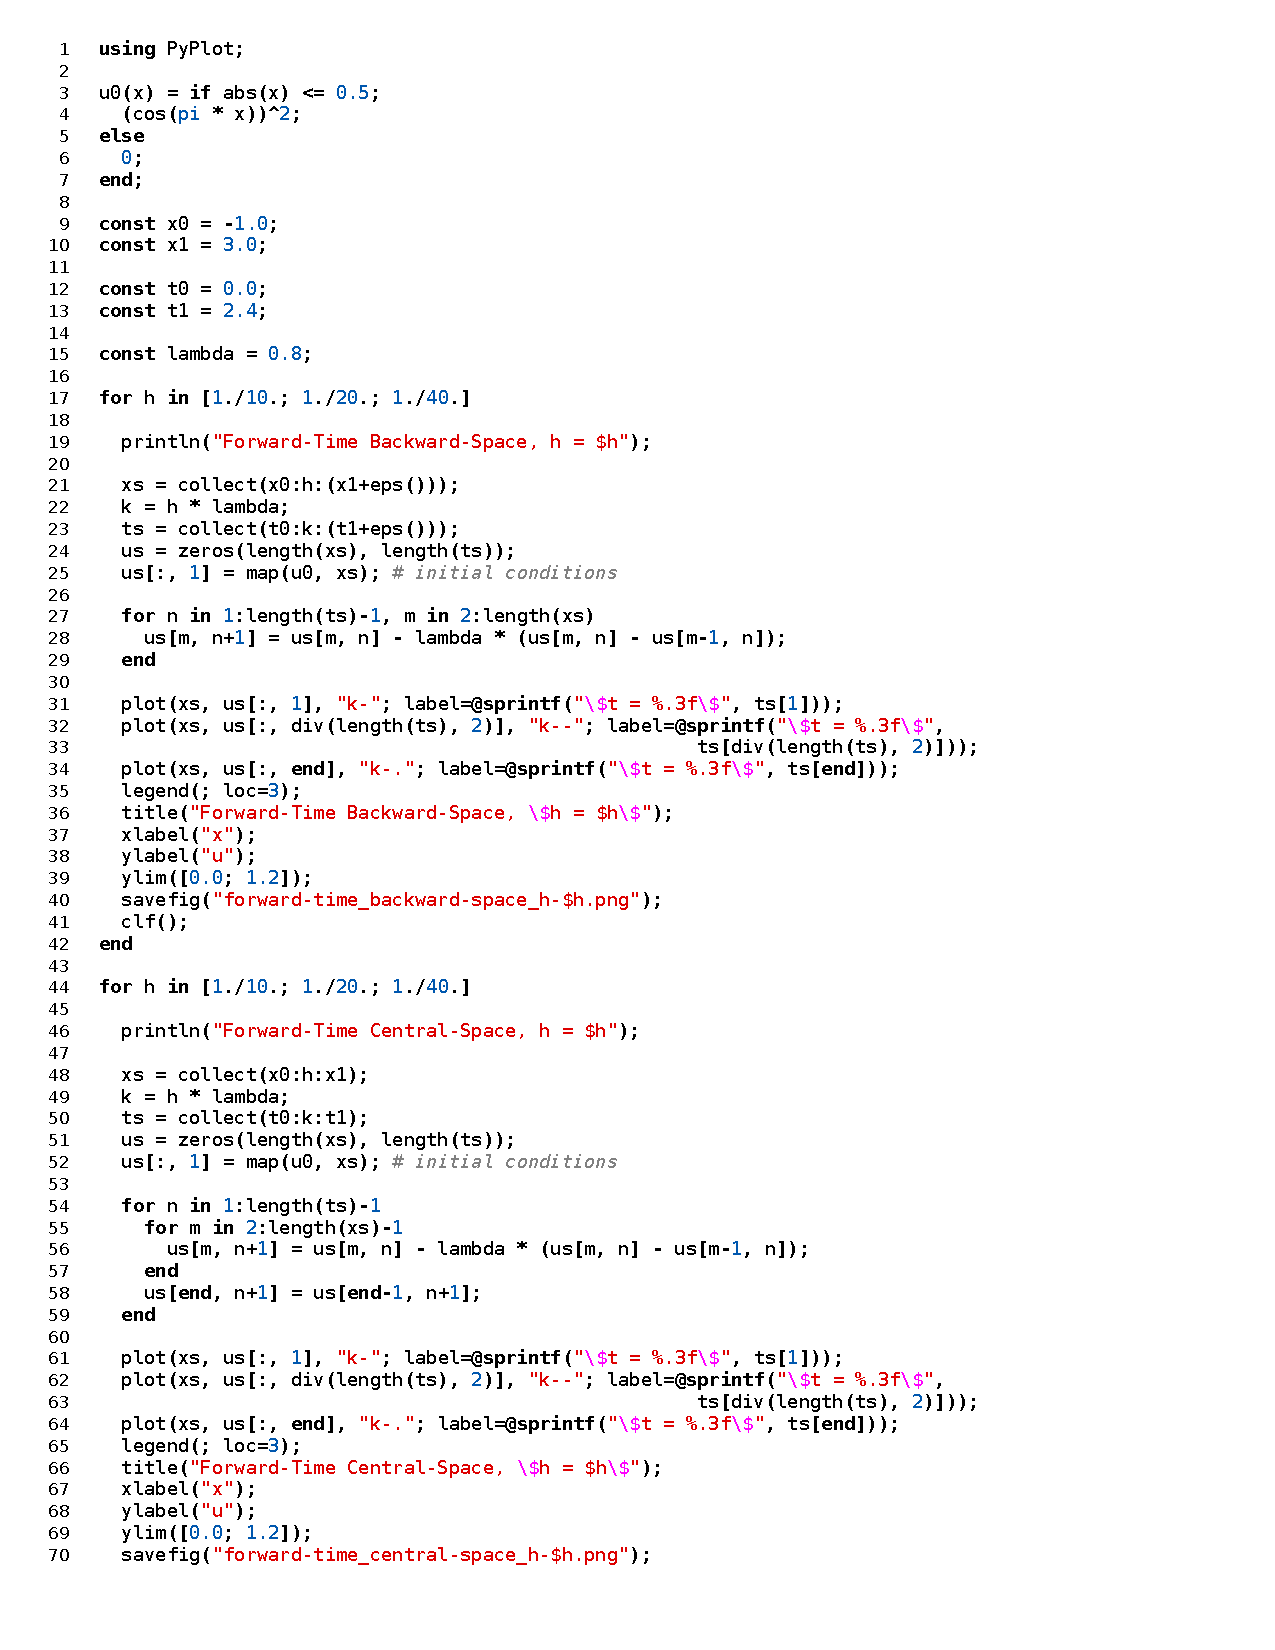
\includepdf[pages=-]{./hw3_code.pdf}
	
\end{document}